\chapter{The Euclid photometric survey}
\label{appendix1-mnu}

Angular power spectra, depending on two redshifts $z_i$ and $z_j$, can be written as integrals of transfer functions $\Delta_{\ell}^i(k)$ over wavenumbers $k$:
\begin{equation} \label{eq:Cl}
C_{\ell}^{ij} = 4\pi \int d\ln k\; \mathcal{P}_{\mathcal{R}}(k) \Delta_{\ell}^{i}(k) \Delta_{\ell}^{i}(k) \;.
\end{equation}
Here $\mathcal{P}_{\mathcal{R}}(k)=A_s k^{n_s-1}$ is the primordial power spectrum of curvature perturbations.
The transfer functions $\Delta_{\ell}^i(k)$ include an integral over a window function $W_i(z)$ describing the binning in redshift, multiplied by the number of galaxies per redshift interval $dN/dz$:
\begin{equation} \label{eq:Delta_l}
  \Delta_{\ell}^i(k) = \int dz\; \frac{dN}{dz} W_i(z) \Delta_{\ell}(z,k) \;.
\end{equation}
%
The main contributions to the transfer functions $\Delta_{\ell}(z,k)$ appearing in the integral of Eq.~(\ref{eq:Delta_l}) are given by the intrinsic galaxy density perturbation, redshift space distortions and lensing effects:
\begin{eqnarray}
  \Delta_{\ell}(z,k) &=& b_G(z) \delta(z,k) j_\ell(kr(z))
  + \frac{k}{\cal H} V(z,k) \frac{d^2 j_\ell(kr(z))}{d(kr(z))^2}
  \nonumber \\
  &&+ \left( \frac{2-5s}{2}\right) \ell(\ell+1)
  \nonumber \\
  &&\times \int_0^{r(z)} d\tilde r\; \frac{r(z)-{\tilde r}}{r(z) {\tilde r}} \left[ {\Phi}(\tilde z,k) + {\Psi}(\tilde z,k) \right] j_\ell(k{\tilde r}) \;.
  \nonumber \\
\end{eqnarray}
We introduced the Fourier transforms of the density perturbations (in comoving gauge), of the metric perturbations $\Phi$, $\Psi$ and of the velocity potential, $v_i\equiv-\partial_i V$, in the Newtonian gauge\footnote{With initial conditions such that ${\cal R}(z_{\rm{in}},k)=1$.}.
The functions $j_\ell(kr(z))$ denote the spherical Bessel functions.
The integral along the line of sight describes the effects of lensing convergence which affects number counts by magnifying the sources, and hence affecting their number density per steradian.
The factor $s(z)$ is called magnification bias and it depends on the luminosity function of the given galaxy population.
Note that for the special value $s=2/5$, lensing has no effect on number counts, while it as opposite sign for larger or smaller values, respectively.


\begin{figure}[t!]
\vspace{0.3cm}
\begin{center}
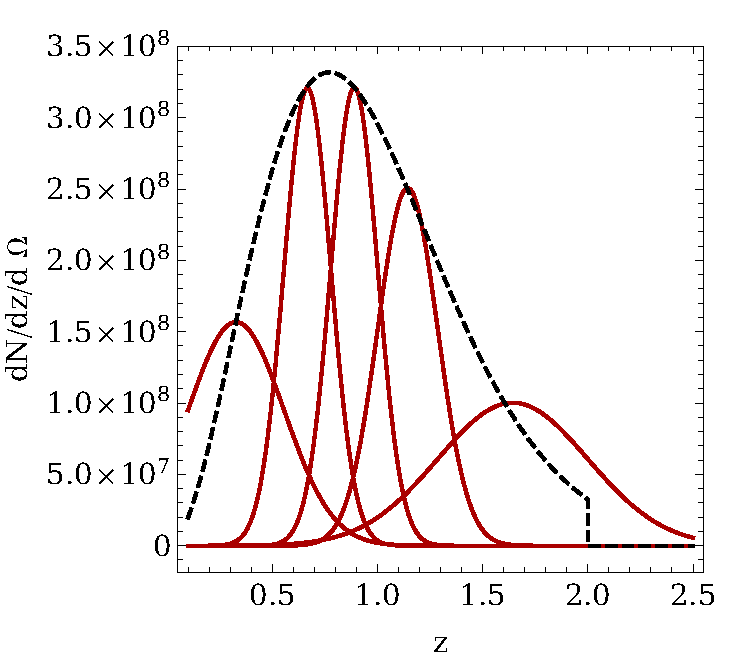
\includegraphics[width=.45\textwidth]{figures/chapter-mnu/euclid_5bin.pdf}
\end{center}
\caption{Euclid photometric galaxy density distribution (black line) with a division into 5 bins containing the same number of galaxies.
}
\label{fig:dNdz}
\end{figure}

%
\begin{figure}[t!]
\begin{center}
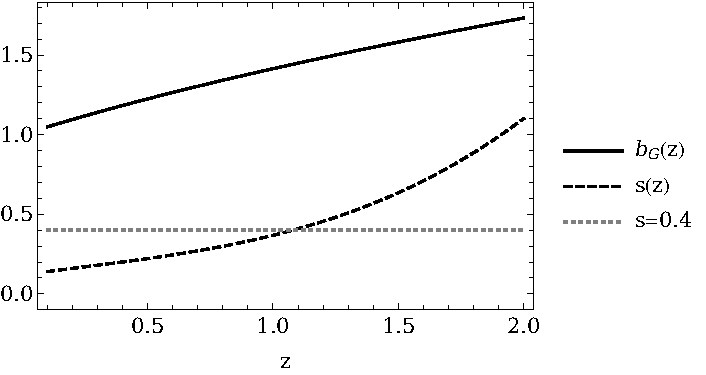
\includegraphics[width=.45\textwidth]{figures/chapter-mnu/bs.pdf}
\end{center}
\caption{Galaxy bias $b_G(z)$ and magnification bias $s(z)$ for Euclid. The
magnification bias is computed at the limiting magnitude $m_{\rm lim}=24.5$.
As a reference, we also plot the value $s=0.4$ at which the lensing contribution to number counts changes sign.
}
\label{fig:bs}
\end{figure}
%

Following \cite{EuclidRB,Amendola:2016saw}, we consider Euclid photometric specifications and approximate the number of galaxies per redshift and per steradian, the galaxy density, the covered sky fraction, the galaxy bias and magnification bias as
\bea
&&\frac{dN}{dzd\Omega} = 3.5\times10^8 z^2 \exp\left[-\left( \frac{z}{z_0} \right)^{3/2}\right] \; \\
&&\quad \mbox{for} \quad 0<z<2.0\;, \nonumber \\
&&d=30\mbox{ arcmin}^{-2}\;,\\
&&f_{\rm sky}=0.364\;,\\
&&b_G(z)=b_0\sqrt{1+z}\;,\\
&&s(z)=s_0 + s_1 z + s_2 z^2 + s_3 z^3 \;. \label{eq:sz_euclid}
\eea
where $z_0=z_{\rm mean}/1.412$ and the median redshift is $z_{\rm mean}=0.9$.
We set $b_0=1$ in our fiducial model and then vary it in the MCMC chains.
The magnification bias is computed in Ref.~\cite{Montanari:2015rga} and the coefficients are $s_0=0.1194$, $s_1=0.2122$, $s_2=-0.0671$ and $s_3=0.1031$.
Figure~\ref{fig:dNdz} shows the division into 5 Gaussian bins containing the same number of galaxies.
For numerical convenience we set the lower redshift bound to $z=0.1$; this affects  our results by a negligible amount.
Figure~\ref{fig:bs} shows the redshift dependence of galaxy and magnification bias. We assume constant galaxy bias and magnification bias within each bin, the values being determined by the mean redshift of the bin.
